Assuming that data is appropriately treated to eliminate redundant
features, we proceed to propose surrogate models and criteria
used for their evaluation. The task all presented surrogates strive to solve can be
formulated using the language of conventional regression problems. In this section,
we focus on interpretation in the scheme of supervised learning with decoupled
and adaptive sampling.

Labeling the expensive MC TBR model $f(x)$, a surrogate is a mapping
$\hat{f}(x)$ that yields similar images as $f(x)$. In other words, $f(x)$ and
$\hat{f}(x)$ minimise a selected dissimilarity metric. Furthermore, in order to
be considered \textit{viable}, surrogates are required to achieve expected evaluation time
lower than that of $f(x)$.

In the decoupled sampling approach that is further described
in~\cref{sec:supervised}, we first gather a sufficiently large
training set of samples $\mathcal{T}=\left\{\left( x^{(i)},f\left(x^{(i)}\right) \right)\right\}_{i=1}^N$
to describe the behaviour of $f(x)$ across its domain.
Depending on specific model family and appropriate choice of its
hyperparameters, surrogate models $\hat{f}(x)$ are trained to minimise
the empirical risk~$R_{\text{emp.}}$ with respect to $\mathcal{T}$ and a model-specific
loss function $\mathcal{L}$, where the empirical risk is defined as
$R_{\text{emp.}}(\hat{f}\mid\mathcal{T},\mathcal{L})
	=\frac{1}{N}\sum_{i=1}^N
	\mathcal{L}\left(\hat{f}(x^{(i)}),f(x^{(i)})\right)$.


The adaptive sampling approach that we characterise in~\cref{sec:adaptive} can be viewed as a more general problem.
Rather than fixing the training set $\mathcal{T}$ for the entire duration of
training, multiple sets $\{\mathcal{T}_k\}_{k=0}^K$ are used, such that
$\mathcal{T}_{k-1}\subset\mathcal{T}_k$ for all $k>1$. The first set
$\mathcal{T}_0$ is initialised randomly to provide a \textit{burn-in}, and is
repeatedly extended in epochs, whereby each epoch trains a new surrogate on
$\mathcal{T}_k$ using the supervised learning procedure, evaluates its
performance, and forms a new set $\mathcal{T}_{k+1}$ by adding more samples to
$\mathcal{T}_k$. This permits the learning algorithm to condition the selection
of new samples on the evaluation results in order to maximise improvement of
surrogate performance over complex regions within the domain.


\subsection{Metrics}
\label{sec:metrics}

Aiming to provide objective comparison of a diverse set of surrogate model
families, we define a multitude of metrics to be tracked during experiments.
Following the motivation of this work, two desirable properties of surrogates
arise: (i) their capability to approximate the TBR MC model well and (ii) their
prediction time. An ideal surrogate would maximise
the former while minimising the latter.

\Cref{tbl:metrics} provides an exhaustive listing and description of metrics recorded
in the experiments. For regression performance analysis, we include a selection
of absolute metrics to assess the approximation capability of surrogates, and set
practical bounds on the expected uncertainty of their predictions. In addition, we also track
relative measures that are better-suited for comparison between this work and others, as
they maintain invariance with respect to the selected domain and image space.
For complexity analysis, surrogates are assessed in terms of wall time
elapsed during training and predicition. This is motivated by common practical use
cases of our work, where models are trained and used as drop-in replacements for the
expensive MC TBR model. Since training set sizes remain to be determined, all times are
reported per a single datapoint. Even though some surrogates support acceleration
by means of parallelisation, measures were taken to ensure sequential
processing of samples to achieve comparability between considered
models.\footnote{The only exception to this are artificial neural networks, which are
notoriously slow to train on conventional CPU architectures in serialised
setting.}

\begin{table}[h]
	\centering
	{\footnotesize
		\begin{tabular}{llrl}
		\toprule
		Regression performance metrics	& Mathematical formulation / description &
		\multicolumn{2}{c}{Ideal value [units]} \\
		\midrule
		Mean absolute error (MAE)	& $\sum_{i=1}^N |y^{(i)}-\hat{y}^{(i)}|/N$ & 0
									& [TBR] \\
		Standard error of regression $S$	& $\text{StdDev}_{i=1}^N\left\{ |y^{(i)} -
		\hat{y}^{(i)}| \right\} $	 & 0 & [TBR] \\
		Coefficient of determination $R^2$	& $1-\sum_{i=1}^N \left(y^{(i)}-\hat{y}^{(i)} \right)^2 /
		\sum_{i=1}^N \left( y^{(i)}-\overline{y} \right)^2 $ & 1 & [rel.] \\
		Adjusted $R^2$	& $1-(1-R^2)(N-1)/(N-P-1)$	& 1 & [rel.] \\
		\midrule
		Complexity metrics	& {} & {} & {} \\
		\midrule
		Mean training time $\overline{t}_{\text{trn.}}$	& $(\text{wall training time of
		$\hat{f}(x)$})/N_0$ 	& 0 & [ms] \\
		Mean prediction time $\overline{t}_{\text{pred.}}$	& $(\text{wall prediction time of
		$\hat{f}(x)$})/N$	& 0 & [ms] \\
		Relative speedup $\sigma$	& $(\text{wall evaluation time of $f(x)$}) /
		(N\overline{t}_{\text{pred.}})$	&
		$\to\infty$ & [rel.] \\
		\bottomrule
		\end{tabular}
	}
	\caption{Metrics recorded in supervised learning experiments. In
	formulations, we work with a training set of size $N_0$ and a test set of
size $N$, TBR values $y^{(i)}=f(x^{(i)})$ and $\hat{y}^{(i)}=\hat{f}(x^{(i)})$
denote images of the $i$th testing sample in the expensive model and the surrogate
respectively. Furthermore, the mean $\overline{y}=\sum_{i=1}^N y^{(i)}/N$ and $P$ is the
number of input features.}
	\label{tbl:metrics}
\end{table}

To prevent undesirable bias in results due to training set selection, all metrics
are collected in the scheme of $k$-fold cross-validation with a standard choice of
$k=5$. Herein, a sample set is subdivided into 5 disjoint foldsi, each of which
is used as a test set for the model trained on the remaining 4.\footnote{Unless explicitly stated otherwise, we use 1
fold for testing and the $k-1$ remaining folds for training. This gives 80\% to
20\% train-test ratio.} In each such run experiments are
repeated, and the overall value of each metric is reported as the mean and
standard deviation over all folds.


\subsection{Decoupled Sampling}
\label{sec:supervised}

In our experiments, we evaluate and compare surrogates in effort to
optimise against metrics described in~\cref{sec:metrics}. To attain meaningful
and practically usable results, we require a sufficiently large and diverse pool
of surrogate families to draw from. This is described by the listing in~\cref{tbl:surrogates}. The presented selection of models includes basic
techniques suitable for linear regression enhanced by the kernel trick or dimension
lifting, methods driven by decision trees, instance-based learning models,
ensemble regressors, randomized algorithms, artificial neural networks and mathematical approaches
developed specifically for the purposes of surrogate modelling. For each of
these families, a state-of-the-art implementation was selected and adapted to
operate with TBR samples.

\begin{table}[h]
	\centering
	{\footnotesize
		\begin{tabular}{llll}
		\toprule
		Surrogate & Acronym & Implementation & Hyperparameters \\
		\midrule
		Support vector machines~\cite{fan2008liblinear}	& SVM & SciKit Learn~\cite{scikit-learn} & 3 \\
		Gradient boosted trees~\cite{friedman2001greedy,friedman1999stochastic,hastie2009elements}	& GBT & SciKit Learn & 11 \\
		Extremely randomized trees~\cite{geurts2006extremely}	& ERT & SciKit Learn & 7 \\
		AdaBoosted decision trees~\cite{drucker1997improving}	& ABT & SciKit Learn & 3 \\
		Gaussian process regression~\cite{williams2006gaussian}	& GPR & SciKit Learn & 2 \\
		$k$ nearest neighbours	& KNN & SciKit Learn & 3 \\
		Artificial neural networks	& ANN & Keras (TensorFlow)~\cite{chollet2015keras} & 2 \\
		Inverse distance weighing~\cite{shepard1968two} & IDW & SMT~\cite{SMT2019} & 1 \\
		Radial basis functions & RBF & SMT & 3 \\
		\bottomrule
		\end{tabular}
	}
	\caption{Considered surrogate model families.}
	\label{tbl:surrogates}
\end{table}

While some of the presented model families are clearly determined by an explicit
choice of a learning algorithm, others may vary considerably depending on
hyperparameter configuration. A good example of the latter group are artificial neural
networks, which in addition to conventional hyperparameters enable to control network
architecture through selection from various parametric graph templates
(see~\cref{fig:nn-archs} for details). This allows us to realise a simplistic
network architecture search during the hyperparameter optimisation procedure.

\begin{figure}[h]
	\centering
	\begin{subfigure}[b]{0.25\textwidth}
		\centering
		{\scriptsize \incfigscale{0.6}{1h3f}}
		\caption{$\text{1h3f}(W)$}
	\end{subfigure}\hfill%
	\begin{subfigure}[b]{0.25\textwidth}
		\centering
		{\scriptsize \incfigscale{0.6}{kf}}
		\caption{$\text{df}(D,W)$}
	\end{subfigure}\hfill%
	\begin{subfigure}[b]{0.25\textwidth}
		\centering
		{\scriptsize \incfigscale{0.6}{3pyramid}}
		\caption{$\text{3pyramid}(W)$}
	\end{subfigure}\hfill%
	\begin{subfigure}[b]{0.25\textwidth}
		\centering
		{\scriptsize \incfigscale{0.6}{5diam}}
		\caption{$\text{5diamond}(W)$}
	\end{subfigure}

	\caption{Selected parametric neural network architectures. All layers except
		the last use ReLU activation. Prediction information flow is indicated by
		arrows.}
	\label{fig:nn-archs}
\end{figure}

\subsubsection{Experiments}
\label{sec:experiment-methodology}

The presented surrogate candidates are evaluated in four experimental cases:%
\begin{enumerate}
	\item Hyperparameter tuning in a simplified domain.

	\item Hyperparameter tuning in full domain.

	\item Scaling benchmark.

	\item Model comparison.
\end{enumerate}

The aim of the initial experiments is to use a relatively small subset of
collected TBR samples to determine hyperparameters of considered surrogates.
Since this process requires learning the behaviour of an unknown, possibly
expensive mapping---here a function that assigns cross-validated metrics to a
point in the hyperparameter domain---it in many aspects mirrors
the primary task of this work with the notable extension of added utility
to optimise. In order to avoid undesirable exponential slowdown in exhaustive
searches of a possibly high-dimensional parameter space, Bayesian
optimisation is employed as a standard hyperparameter tuning algorithm. We set
its objective to maximise $R^2$ and perform
1000~iterations.\footnote{Hyperparameter tuning of each surrogate family was
	terminated after 2~days. Instances that reached this limit may be identified
	in~\cref{tbl:exp1-detailed-results,tbl:exp2-detailed-results}.}

In the first experiment, efforts are made to maximise the possibility of success
in surrogates that are prone to suboptimal performance in discontinuous spaces.
This follows the notion that, if desired, performance of such models may be
replicated by training separate instances to model each continuous subregion of
the domain independently.
To this end, data are limited to a single slice from run~2, and discrete
features are completely withheld from evaluated
surrogates. This is repeated for each of the four available slices to
investigate variance in behaviour under different discrete feature assignments.
The second experiment conventionally measures surrogate performance on the full
feature space. Here, in extension of the previous case, surrogates work with
samples comprised of discrete as well as continuous features.

The goal of the last two experiments is to exploit the information gathered by
hyperparameter tuning to investigate scaling properties. In
the third experiment, the 20~best-performing hyperparameter choices of each family
(in $R^2$) are used to learn surrogates using progressively larger training sets. Following
that, the fourth experiment aims to produce surrogates for practical use by
retraining selected well-scaling models to further optimise their properties.


\subsection{Adaptive Sampling}
\label{sec:adaptive}

All of the surrogate modelling techniques studied in this project face a shared
challenge: their accuracy is limited by the quantity of training samples which
are available from the expensive MC TBR model. Adaptive sampling procedures can
improve upon this limitation by taking advantage of statistical information
which is accumulated during the training of any surrogate model. Rather than
training the surrogate on a single sample set generated according to a fixed
strategy, sample locations are chosen incrementally so as to best suit the model
under consideration.

Adaptive sampling techniques are widespread in the literature and have been
specialised for surrogate modelling. Garud's \cite{Garud2016} "Smart Sampling
Algorithm" achieved notable success by incorporating surrogate quality and
crowding distance scoring to identify optimal new samples, but was only tested
on a single-parameter domain. We theorised that a nondeterministic sample
generation approach, built around Markov Chain Monte Carlo methods (MCMC), would
fare better for high-dimensional models by more thoroughly exploring all local
optima in the feature space. MCMC produces a progressive chain of sample points,
each drawn according to the same symmetric proposal distribution
from the prior point. These sample points will converge to a desired posterior
distribution, so long as the acceptance probability for these draws has a
particular functional dependence on that posterior value (see \cite{Zhou2018}
for a review).

%\footnote{An
%adaptive MCMC procedure \cite{Zhang2012}, which adjusts an ellipsoidal proposal
%distribution to fit the posterior, was also implemented but not fully tested.}

Many researchers have embedded surrogate methods into MCMC strategies for
parameter optimisation \cite{Zhang2020,Gong2017}, in particular the ASMO-PODE
algorithm \cite{Ginting2011} which makes use of MCMC-based adaptive sampling to
attain greater surrogate precision around prospective optima. Our novel approach
draws inspiration from ASMO-PODE, but instead uses MCMC to generate samples
which increase surrogate precision throughout the entire parameter space.

\begin{wrapfigure}{r}{0.55\textwidth}
  \vspace{-35pt}
  \begin{center}
    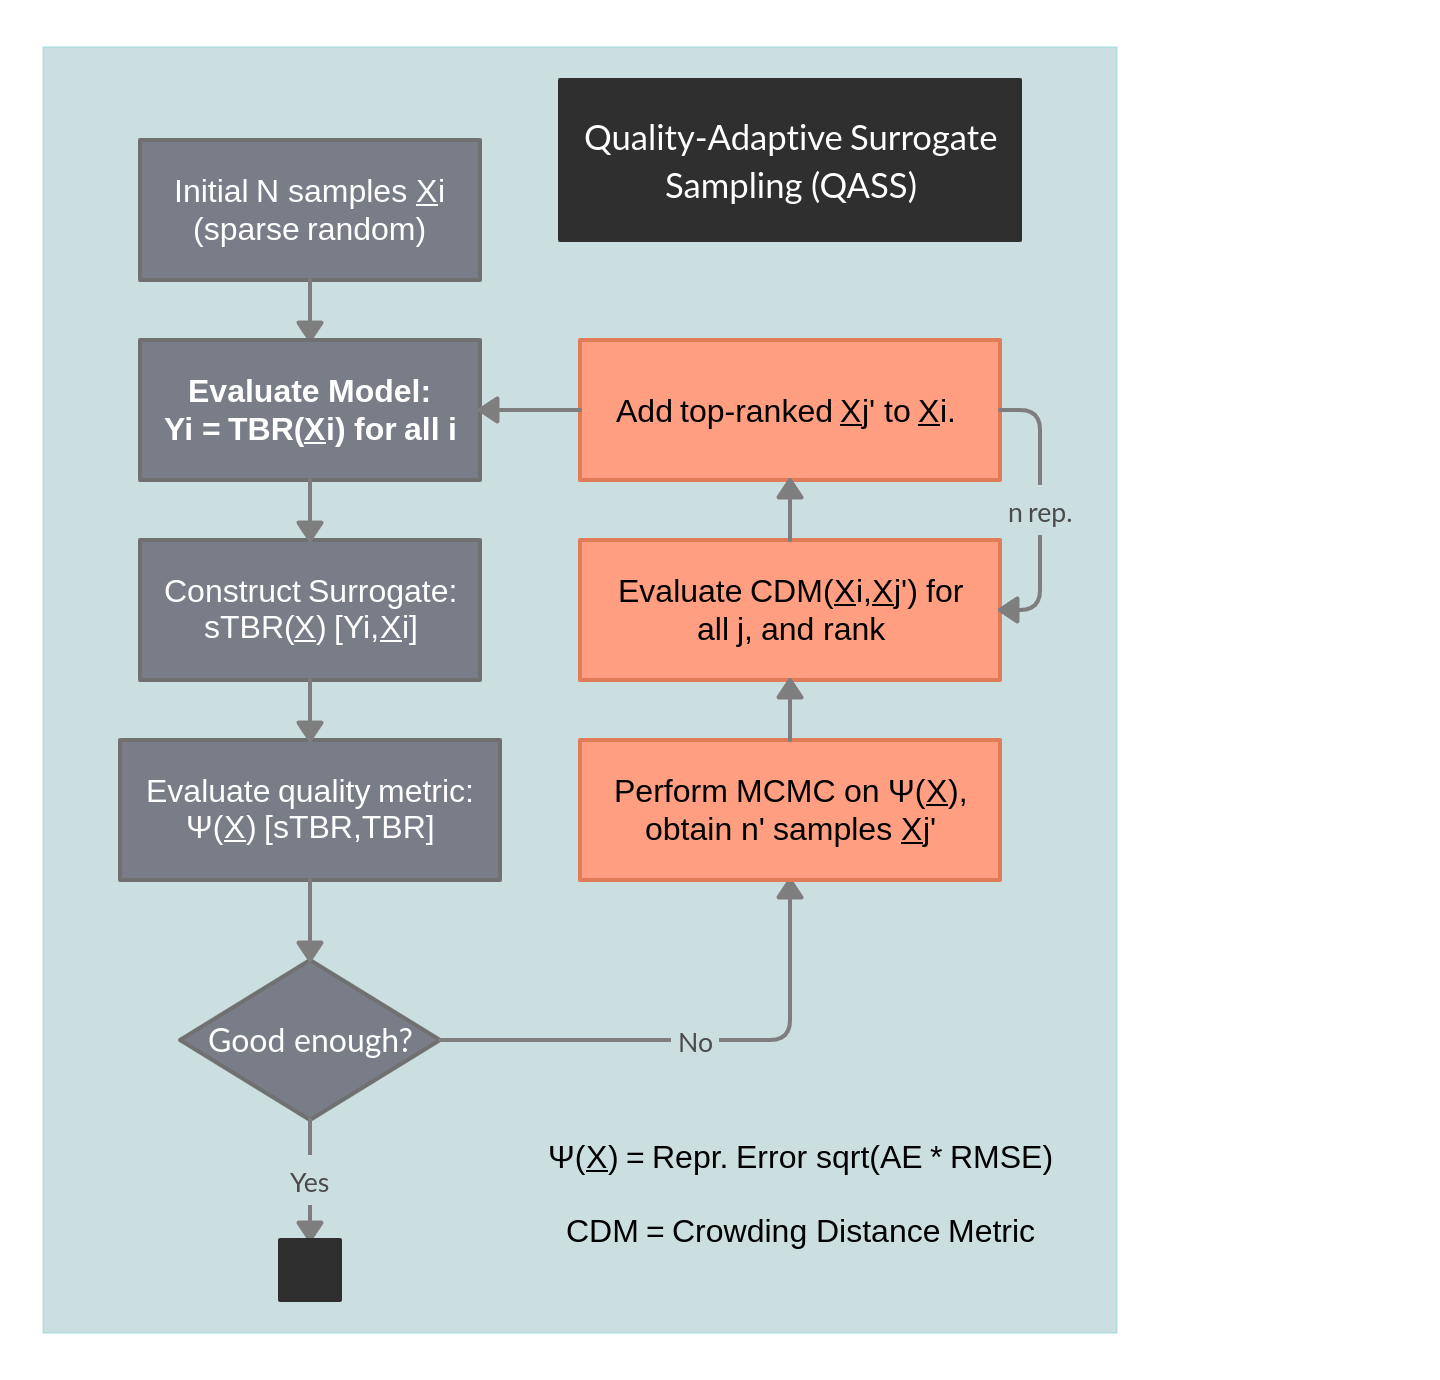
\includegraphics[width=0.7\textwidth]{fig4_qassplan.png}
    \caption{Schematic of QASS algorithm}
    \label{fig:qassplan}
  \end{center}
  \vspace{-80pt}
\end{wrapfigure}

% TODO: explain AE

We designed the Quality-Adaptive Surrogate Sampling algorithm (QASS,
\cref{fig:qassplan}) to iteratively increment the training/test set with sample
points which maximise surrogate error and minimise a crowding distance metric
(CDM) \cite{Solonen2012} in feature space. On each iteration following an initial training of the surrogate on $N$ uniformly random samples, the surrogate was trained and AE calculated. MCMC was then performed on the error function generated by performing nearest-neighbor interpolation on these test error points. The resultant samples were culled by $50\%$ according to the CDM, and then the $n$ highest-error candidates were selected for reintegration with the training/test set, beginning another training epoch. Validation was also performed during each iteration on independent, uniformly-random sample sets.

% Adaptive multi-chain MCMC: \cite{Zhang2012}



